{
\newcommand{\thisscale}{0.8}

\newcommand{\nodebase}[1]{\begin{tikzpicture}[node/.style = {shape=circle},scale=\thisscale, every node/.style={scale=\thisscale}]
\useasboundingbox (0,-0.15) circle (.45);
\node at (0,0) {$\Av{132}$};
\node at (0,-0.4) {\tiny #1};
\end{tikzpicture}}

\newcommand{\nodepos}[1]{\begin{tikzpicture}[node/.style = {shape=circle},scale=\thisscale, every node/.style={scale=\thisscale}]
\useasboundingbox (0,-0.15) circle (.55);
\node at (0,0) {$\textsf{Av}_{\geq1}(132)$};
\node at (0,-0.45) {\tiny #1};
\end{tikzpicture}}

\newcommand{\nodeposempty}{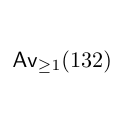
\begin{tikzpicture}[node/.style = {shape=circle},scale=\thisscale, every node/.style={scale=\thisscale}]
\useasboundingbox (0,0) circle (.55);
\node at (0,0) {$\textsf{Av}_{\geq1}(132)$};
\end{tikzpicture}}

\newcommand{\nodeneut}[1]{\begin{tikzpicture}[node/.style = {shape=circle},scale=\thisscale, every node/.style={scale=\thisscale}]
\useasboundingbox (0,-0.15) circle (.45);
\node at (0,0) {$\set{\varepsilon}$};
\node at (0,-0.45) {\tiny \underline{\underline{#1}}};
\end{tikzpicture}}

\newcommand{\nodeatom}[1]{\begin{tikzpicture}[node/.style = {shape=circle},scale=\thisscale, every node/.style={scale=\thisscale}]
\useasboundingbox (0,-0.15) circle (.45);
\node at (0,0) {$\set{\tikz{\fill (0,0) circle (0.1);}}$};
\node at (0,-0.45) {\tiny \underline{\underline{#1}}};
\end{tikzpicture}}

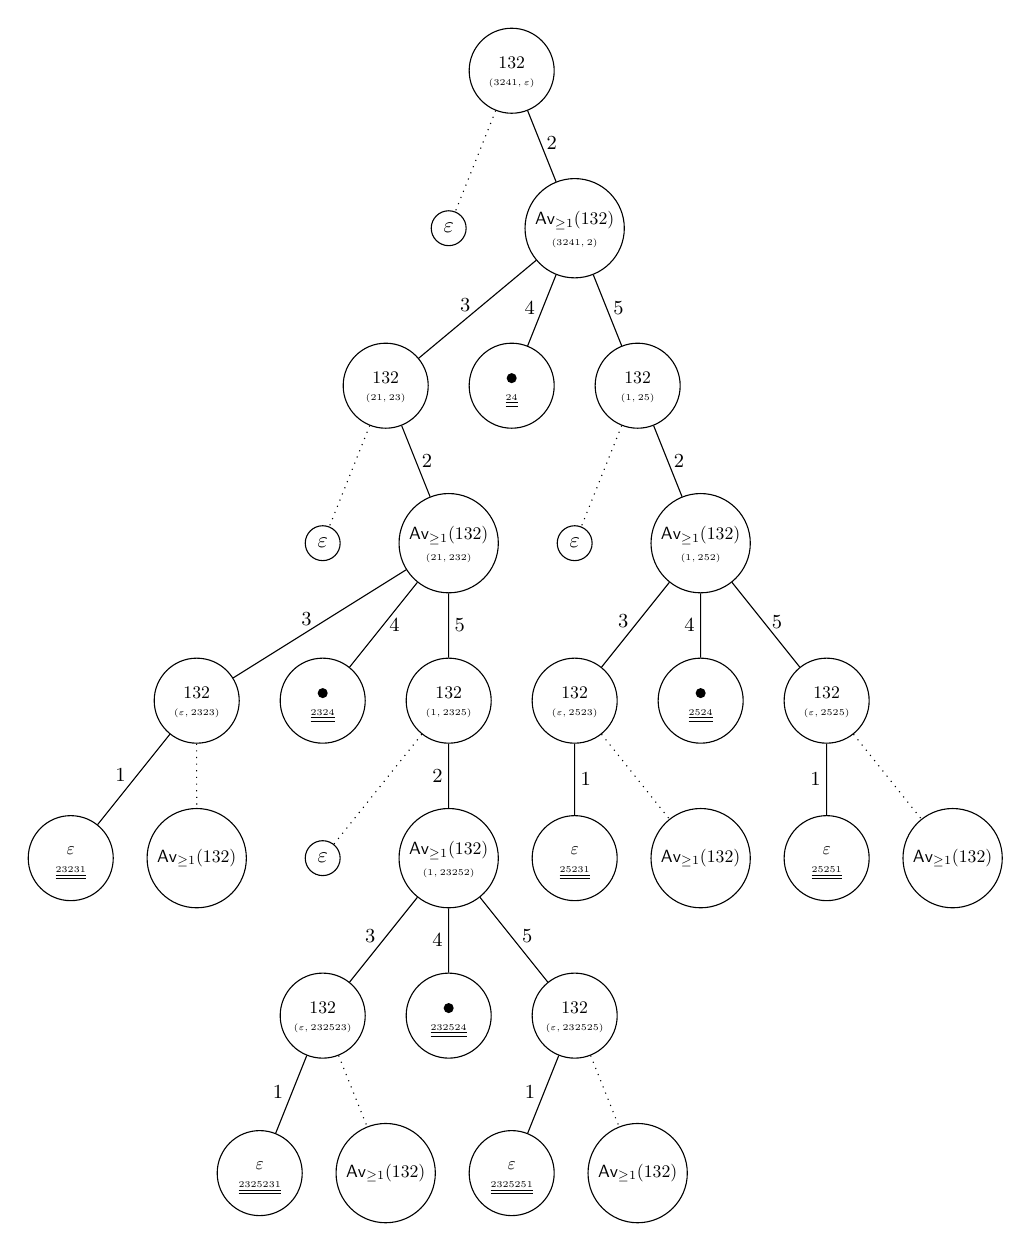
\begin{tikzpicture}[vertex/.style = {shape=circle,draw,minimum size=.5em},scale=\thisscale, every node/.style={scale=\thisscale}]
    \node[vertex] (lvl0) at (0,0) {\nodebase{$(3241,\varepsilon)$}};
    
    \node[vertex] (lvl11) at (-1,-2.5) {$\set{\varepsilon}$};
    \draw[dotted] (lvl0) -- (lvl11);
    \node[vertex] (lvl12) at (1,-2.5) {\nodepos{$(3241,2)$}};
    \draw (lvl0) -- (lvl12) node[pos=.5,xshift=4.5,yshift=1.5] {\small $2$};
    
    \node[vertex] (lvl21) at (-2,-5) {\nodebase{$(21,23)$}};
    \draw (lvl12) -- (lvl21) node[pos=.5,xshift=-5.5,yshift=2] {\small $3$};
    \node[vertex] (lvl22) at (0,-5) {\nodeatom{$24$}};
    \draw (lvl12) -- (lvl22) node[pos=.5,xshift=-5.5,yshift=1] {\small $4$};
    \node[vertex] (lvl23) at (2,-5) {\nodebase{$(1,25)$}};
    \draw (lvl12) -- (lvl23) node[pos=.5,xshift=5,yshift=1] {\small $5$};
    
    \node[vertex] (lvl31) at (-3,-7.5) {$\set{\varepsilon}$};
    \draw[dotted] (lvl21) -- (lvl31);
    \node[vertex] (lvl32) at (-1,-7.5) {\nodepos{$(21,232)$}};
    \draw (lvl21) -- (lvl32) node[pos=.5,xshift=5,yshift=0] {\small $2$};
    \node[vertex] (lvl33) at (1,-7.5) {$\set{\varepsilon}$};
    \draw[dotted] (lvl23) -- (lvl33);
    \node[vertex] (lvl34) at (3,-7.5) {\nodepos{$(1,252)$}};
    \draw (lvl23) -- (lvl34) node[pos=.5,xshift=5,yshift=0] {\small $2$};
    
    \node[vertex] (lvl41) at (-5,-10) {\nodebase{$(\varepsilon,2323)$}};
    \draw (lvl32) -- (lvl41) node[pos=.5,xshift=-6,yshift=2.25] {\small $3$};
    \node[vertex] (lvl42) at (-3,-10) {\nodeatom{$2324$}};
    \draw (lvl32) -- (lvl42) node[pos=.5,xshift=5,yshift=0] {\small $4$};
    \node[vertex] (lvl43) at (-1,-10) {\nodebase{$(1,2325)$}};
    \draw (lvl32) -- (lvl43) node[pos=.5,xshift=5,yshift=0] {\small $5$};
    \node[vertex] (lvl44) at (1,-10) {\nodebase{$(\varepsilon,2523)$}};
    \draw (lvl34) -- (lvl44) node[pos=.5,xshift=-5.5,yshift=1.5] {\small $3$};
    \node[vertex] (lvl45) at (3,-10) {\nodeatom{$2524$}};
    \draw (lvl34) -- (lvl45) node[pos=.5,xshift=-5,yshift=0] {\small $4$};
    \node[vertex] (lvl46) at (5,-10) {\nodebase{$(\varepsilon,2525)$}};
    \draw (lvl34) -- (lvl46) node[pos=.5,xshift=5,yshift=1] {\small $5$};
    
    \node[vertex] (lvl51) at (-7,-12.5) {\nodeneut{$23231$}};
    \draw (lvl41) -- (lvl51) node[pos=.5,xshift=-6,yshift=2] {\small $1$};
    \node[vertex] (lvl52) at (-5,-12.5) {\nodeposempty};
    \draw[dotted] (lvl41) -- (lvl52);
    \node[vertex] (lvl53) at (-3,-12.5) {$\set{\varepsilon}$};
    \draw[dotted] (lvl43) -- (lvl53);
    \node[vertex] (lvl54) at (-1,-12.5) {\nodepos{$(1,23252)$}};
    \draw (lvl43) -- (lvl54) node[pos=.5,xshift=-5,yshift=0] {\small $2$};;
    \node[vertex] (lvl55) at (1,-12.5) {\nodeneut{$25231$}};
    \draw (lvl44) -- (lvl55) node[pos=.5,xshift=5,yshift=0] {\small $1$};
    \node[vertex] (lvl56) at (3,-12.5) {\nodeposempty};
    \draw[dotted] (lvl44) -- (lvl56);
    \node[vertex] (lvl57) at (5,-12.5) {\nodeneut{$25251$}};
    \draw (lvl46) -- (lvl57) node[pos=.5,xshift=-5,yshift=0] {\small $1$};
    \node[vertex] (lvl58) at (7,-12.5) {\nodeposempty};
    \draw[dotted] (lvl46) -- (lvl58);
    
    \node[vertex] (lvl61) at (-3,-15) {\nodebase{$(\varepsilon,232523)$}};
    \draw (lvl54) -- (lvl61) node[pos=.5,xshift=-6,yshift=1.5] {\small $3$};
    \node[vertex] (lvl62) at (-1,-15) {\nodeatom{$232524$}};
    \draw (lvl54) -- (lvl62) node[pos=.5,xshift=-5,yshift=0] {\small $4$};
    \node[vertex] (lvl63) at (1,-15) {\nodebase{$(\varepsilon,232525)$}};
    \draw (lvl54) -- (lvl63) node[pos=.5,xshift=6,yshift=1.5] {\small $5$};
    
    \node[vertex] (lvl71) at (-4,-17.5) {\nodeneut{$2325231$}};
    \draw (lvl61) -- (lvl71) node[pos=.5,xshift=-6,yshift=1] {\small $1$};
    \node[vertex] (lvl72) at (-2,-17.5) {\nodeposempty};
    \draw[dotted] (lvl61) -- (lvl72);
    \node[vertex] (lvl73) at (0,-17.5) {\nodeneut{$2325251$}};
    \draw (lvl63) -- (lvl73) node[pos=.5,xshift=-6,yshift=1] {\small $1$};
    \node[vertex] (lvl74) at (2,-17.5) {\nodeposempty};
    \draw[dotted] (lvl63) -- (lvl74);
\end{tikzpicture}

}